\documentclass[aspectratio=169,10pt]{beamer}
\usetheme{default}
\usepackage{tikz}
\usepackage{array}
\usetikzlibrary{arrows.meta, positioning, fit, backgrounds}
\setbeamertemplate{navigation symbols}{}

% --- Fermilab-ish minimal look: white bg, blue sans titles, thin footer ------
\definecolor{fnalblue}{RGB}{0,84,159}
\definecolor{boxblue}{RGB}{40,90,160}
\definecolor{okgreen}{RGB}{0,130,60}
\setbeamercolor{frametitle}{fg=fnalblue}
\setbeamerfont{frametitle}{size=\Large,series=\bfseries}
\setbeamercolor{structure}{fg=fnalblue}
\setbeamertemplate{frametitle}{\vspace{0.4em}\insertframetitle\par}
\setbeamertemplate{footline}{%
  \hbox{\begin{beamercolorbox}[wd=\paperwidth,ht=2.5ex,dp=1.5ex,leftskip=1em,rightskip=1em]{}%
  \tiny\color{fnalblue}\insertdate\hfill Mu2e Genesis Meeting\hfill\insertframenumber%
  \end{beamercolorbox}}}
\setbeamercolor{itemize item}{fg=fnalblue}
\setbeamercolor{itemize subitem}{fg=fnalblue}

\newcolumntype{W}[1]{>{\raggedright\arraybackslash}p{#1}}

\title{\textcolor{fnalblue}{\textbf{Mu2e Genesis: Agentic Experiment Optimization}}}
\subtitle{\textcolor{fnalblue}{Workflow (i) --- activities and near-term plan (detailed)}}
\author{Y.\ Oksuzian}
\institute{Argonne National Laboratory}
\date{8/6/2026}

\begin{document}

% ------------------------------------------------------------------ title
\begin{frame}[plain]
\vspace{2.2em}
\begin{center}
{\LARGE\bfseries\color{fnalblue} Mu2e Genesis: Agentic Experiment Optimization}\\[0.8em]
{\large\color{fnalblue} Workflow (i) --- activities and near-term plan}\\[0.4em]
{\small\color{fnalblue} detailed version --- see the short deck for the talk}\\[3.0em]
{\large Y.\ Oksuzian}\\[0.3em]
{\large Argonne National Laboratory}\\[0.3em]
{\large Aug.\ 06, 2026}
\end{center}
\end{frame}

% ------------------------------------------------------- architecture loop
\begin{frame}{Agentic Experiment Optimization --- the loop}
\begin{center}
\textcolor{red}{\footnotesize Prompt-to-configuration: simulate, analyze, score, decide --- with a human gate.}
\end{center}
\vspace{-0.3em}
\begin{center}
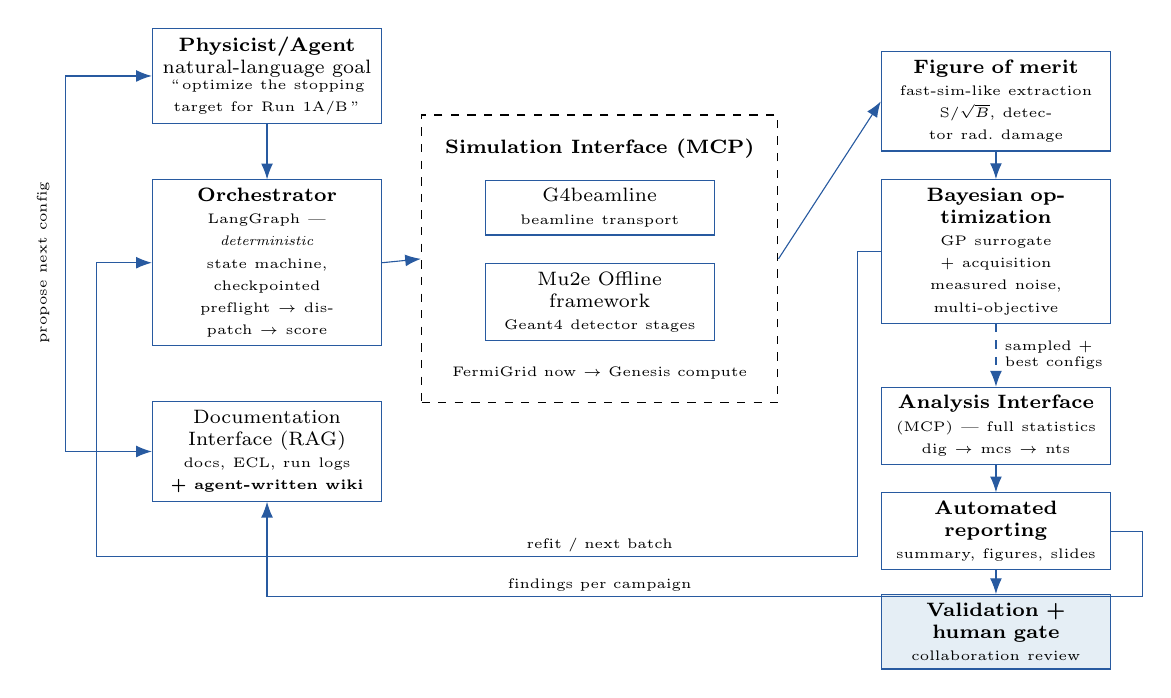
\begin{tikzpicture}[
  font=\scriptsize,
  box/.style={draw=boxblue, rectangle, align=center, inner sep=3pt, text width=27mm},
  grp/.style={draw=black, dashed, rectangle, inner sep=5pt},
  ar/.style={-{Latex[length=2mm]}, draw=boxblue}]

% --- left column: prompt -> agent -> docs
\node[box] (prompt) {\textbf{Physicist/Agent}\\natural-language goal\\{\tiny ``\,optimize the stopping\\target for Run 1A/B\,''}};
\node[box, below=7mm of prompt] (agent) {\textbf{Orchestrator}\\{\tiny LangGraph --- \emph{deterministic}}\\{\tiny state machine, checkpointed}\\{\tiny preflight $\rightarrow$ dispatch $\rightarrow$ score}};
\node[box, below=7mm of agent] (docs) {Documentation\\Interface (RAG)\\{\tiny docs, ECL, run logs}\\{\tiny \textbf{+ agent-written wiki}}};

% --- middle column: the Simulation Interface WRAPS both simulation engines
\node[box, right=13mm of agent, yshift=7mm] (g4bl) {G4beamline\\{\tiny beamline transport}};
\node[box, below=3.5mm of g4bl] (offline) {Mu2e Offline framework\\{\tiny Geant4 detector stages}};
\node[font=\scriptsize\bfseries, above=1.5mm of g4bl] (simtitle) {Simulation Interface (MCP)};
\node[font=\tiny, below=2mm of offline] (compute) {FermiGrid now $\rightarrow$ Genesis compute};
\begin{scope}[on background layer]
\node[grp, fit=(simtitle)(g4bl)(offline)(compute)] (simgrp) {};
\end{scope}

% --- right column: the FAST loop (FoM -> surrogate), then the gated
%     validation branch (full analysis chain on selected configs only)
\node[box, right=13mm of simgrp.east, yshift=20mm] (fom) {\textbf{Figure of merit}\\{\tiny fast-sim-like extraction}\\{\tiny S/$\sqrt{B}$, detector rad.\ damage}};
\node[box, below=3.5mm of fom] (gp) {\textbf{Bayesian optimization}\\{\tiny GP surrogate $+$ acquisition}\\{\tiny measured noise, multi-objective}};
\node[box, below=8mm of gp] (ana) {\textbf{Analysis Interface}\\{\tiny (MCP) --- full statistics}\\{\tiny dig $\rightarrow$ mcs $\rightarrow$ nts}};
\node[box, below=3.5mm of ana] (rep) {\textbf{Automated reporting}\\{\tiny summary, figures, slides}};
\node[box, below=3mm of rep, fill=fnalblue!10] (gate) {\textbf{Validation + human gate}\\{\tiny collaboration review}};

\coordinate (fby) at ([yshift=-7mm]docs.south);

\draw[ar] (prompt) -- (agent);
% Documentation feeds the PROPOSER, not the orchestrator: the state machine is
% deterministic and never queries a doc store (verified -- every wiki mention in
% graph/ is a code comment). The agent reads accumulated findings to propose the
% next configuration, and writes findings back. Routed left, clear of (agent).
\draw[{Latex[length=2mm]}-{Latex[length=2mm]}, draw=boxblue]
      (docs.west) -- ++(-11mm,0) |- (prompt.west);
\node[font=\tiny, rotate=90, anchor=south, align=center]
      at ([xshift=-11.8mm]agent.west) {propose next config};
\draw[ar] (agent.east) -- (simgrp.west);
\draw[ar] (simgrp.east) -- (fom.west);
\draw[ar] (fom) -- (gp);
\draw[ar, dashed] (gp) -- node[right, font=\tiny, align=left, inner sep=3pt] {sampled +\\best configs} (ana);
\draw[ar] (ana) -- (rep);
\draw[ar] (rep) -- (gate);
% SLOW loop (per campaign, knowledge): the batch report writes its findings BACK
% into the documentation store, so the next proposal is informed by what every
% previous batch learned. Implemented today as the wiki/ bundle (Karpathy
% LLM-wiki pattern, OKF v0.1) -- but written by the agent per session, not yet
% emitted automatically at drain. Outer lane, below the fast refit lane.
\coordinate (kby) at ([yshift=-12mm]docs.south);
\draw[ar] (rep.east) -- ++(4mm,0) |- (kby) -- (docs.south);
\node[anchor=south, inner sep=1.5pt] at (simgrp.south |- kby) {\tiny findings per campaign};
% feedback: surrogate -> agent, routed below the diagram
\draw[ar] (gp.west) -- ++(-0.3,0) |- (fby) -| ([xshift=-7mm]agent.west) |- (agent.west);
\node[anchor=south, inner sep=1.5pt] at (simgrp.south |- fby) {\tiny refit / next batch};
\end{tikzpicture}
\end{center}
\end{frame}

% ------------------------------------------------------------- activities 1
\begin{frame}{Activities and owners (1/2)}
\footnotesize
\textbf{Surrogate model optimization} \hfill \textcolor{fnalblue}{(Yuri)}
\begin{itemize}\tiny
  \item GP surrogates over the configuration space; \emph{measured} noise fed to the model; multi-objective acquisition over the true trade: \textbf{sensitivity vs.\ detector radiation damage}
  \item Needed: multi-fidelity, regime-aware objectives, transfer between scenarios, pre-registered predictions to grade the surrogate
  \item \textbf{Explore BO models for higher dimensionality}: TuRBO (rejected at $d{=}6$ --- revisit at 10--12D), SAASBO (sparse axis-aligned; fits our few-dominant-knobs structure), input warping for corner non-stationarity
\end{itemize}
\vspace{0.15em}

\textbf{LangGraph orchestration} \hfill \textcolor{fnalblue}{(Yuri / Ray / Rob)}
\begin{itemize}\tiny
  \item One graph run $=$ one evaluation: propose $\rightarrow$ preflight $\rightarrow$ simulation $\rightarrow$ scoring; checkpointed, resumable, failure-classifying
  \item \textbf{Today the orchestrator is Claude}: LangGraph $+$ Bayesian optimization carry the loop; the LLM agent turns the goal into campaigns, diagnoses failures, decides what runs next. Staying within Claude is a viable option --- the alternative is a KE/MCP orchestrator over the same seams
  \item Needed: expose the loop through MCP; full tool/reasoning traces for reproducibility
  \item \textbf{Parameterize scenarios}: beam intensity, solenoid field scale, arbitrary geometry configuration --- today only geometry knobs are variable, so a new scenario means hand-authoring a mode
\end{itemize}
\vspace{0.15em}

\textbf{Fast sim scoring for Run1A/B} \hfill \textcolor{fnalblue}{(Michael)}
\begin{itemize}\tiny
  \item \textbf{The only scoring path in the loop today}: S/$\sqrt{B}$ and detector radiation damage extracted from the Geant4 output \emph{without} full reconstruction --- what makes search affordable
  \item Needed: \textbf{improve fast-sim performance}; \textbf{revisit Run 1B} (looked at before, needs redoing on the current stack) and new constraint scenarios; quantified agreement with the full analysis chain
  \item \textbf{Explore improvements and other fast-sim options}: beam optics upstream, detector response downstream
\end{itemize}
\end{frame}

% ------------------------------------------------------------- activities 2
\begin{frame}{Activities and owners (2/2)}
\footnotesize
\textbf{Full-sim validation (dig $\rightarrow$ mcs $\rightarrow$ nts)} \hfill \textcolor{fnalblue}{(Sophie / James)}
\begin{itemize}\tiny
  \item \textbf{The high-fidelity path}: full chain at full statistics, autonomously callable --- on selected configurations \emph{and} on a \textbf{sampled fraction (e.g.\ every 10th point)}, run \textbf{asynchronously} so it never blocks the next pick
  \item \textbf{Quantified relationship to the fast score}, and the judgment of whether it is good enough --- sampling spreads paired points across the space, so the calibration comes for free
  \item Needed: per-configuration provenance; the \textbf{evidence bar and sign-off protocol} --- replicates, systematics, background-regime scoping --- before anything reaches collaboration review
\end{itemize}
\vspace{0.15em}

\textbf{Infrastructure --- MCP, LLM, computing} \hfill \textcolor{fnalblue}{(Ray / Rob)}
\begin{itemize}\tiny
  \item MCP servers, model endpoints, and compute allocations
  \item \textbf{Agent skills} --- encoded procedures and gotchas; the proposal's ``orchestration patterns'', a packaged Phase-I artifact
  \item \textbf{Start on FermiGrid, transition to Genesis-provided compute} --- the interfaces should make the backend a swap, not a rewrite
  \item Needed: token and CPU accounting per workflow --- a stated project deliverable
\end{itemize}
\vspace{0.15em}

\textbf{Documentation interface} \hfill \textcolor{fnalblue}{(Cole / Simon)}
\begin{itemize}\tiny
  \item Semantic search over documentation, ECL, shifter logs, run and configuration databases
  \item Needed: context assembly for the \emph{optimizer} --- which constraints are real vs.\ conventional
\end{itemize}
\vspace{0.15em}

\textbf{G4beamline} \hfill \textcolor{fnalblue}{(Yuri)}
\begin{itemize}\tiny
  \item G4beamline MCP server: autonomous configuration, job dispatch, output parsing --- prototype demonstrated, \textbf{a proposal commitment} (App.\ 5)
  \item Needed: \textbf{integrate into the existing workflow} --- the loop runs the Offline framework today; G4beamline plugs into the same seam, no new machinery
\end{itemize}
\vspace{0.15em}

\textbf{Automated reporting} \hfill \textcolor{fnalblue}{(Rob / Yuri)}
\begin{itemize}\tiny
  \item A campaign drains $\rightarrow$ the loop \textbf{summarizes its own results}: regenerates the landscape and geometry figures, rebuilds the deck, and drafts the write-up
  \item \textbf{Write-back}: every campaign appends what it learned to the documentation interface --- an agent-maintained wiki (Karpathy pattern, OKF v0.1). Running today at 125 pages; the write is per session, not yet triggered on drain
  \item Already partly real: figure generators are parameterized per line; today the assembly step is manual
  \item Needed: trigger on drain, \textbf{every number traceable to a leaderboard row}, and a human gate before anything circulates
\end{itemize}

\end{frame}

% ------------------------------------------------------------------ status
\begin{frame}{Status --- the loop runs end-to-end}
\vspace{-0.6em}
\begin{center}
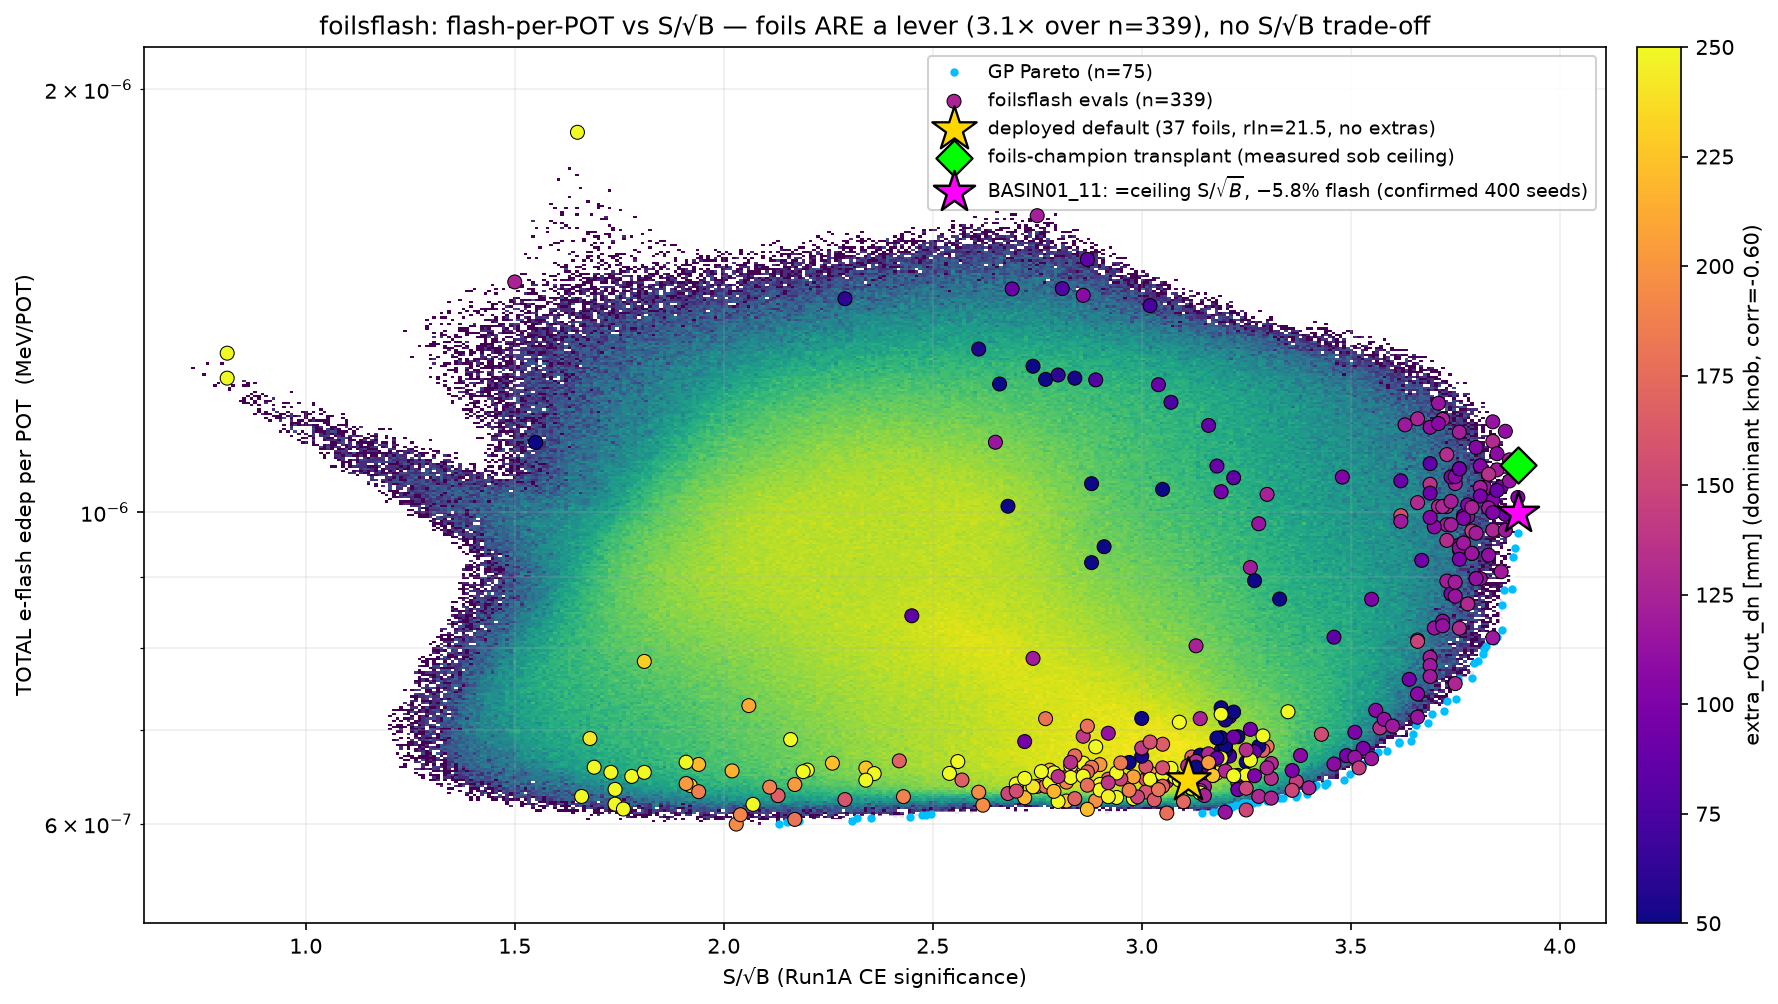
\includegraphics[width=0.60\textwidth]{foilsflash_perpot_cloud_nochamp.png}
\end{center}
\vspace{-0.2em}
\begin{columns}[T]
\begin{column}{0.55\textwidth}
\scriptsize
\begin{tabular}{@{}lcc@{}}
\hline
design & S/$\sqrt{B}$ & rad.\ damage \\
\hline
deployed default & 3.11 & 6.45$\times10^{-7}$ \\
\texttt{ff11R00\_07} (champion) & \textbf{3.31} & \textbf{6.26$\times10^{-7}$} \\
\texttt{ff14R01\_00} (exploit) & 3.84 & 8.14$\times10^{-7}$ \\
\texttt{BASIN01\_11} (confirmed) & \textbf{3.90} & 1.00$\times10^{-6}$ \\
\hline
\end{tabular}
\end{column}
\begin{column}{0.43\textwidth}
\scriptsize
\begin{itemize}\scriptsize
  \item \textbf{339} evaluations map a clean Pareto front
  \item Champion beats deployed on \textbf{both} axes: $+6\%$ S/$\sqrt{B}$ at $-3\%$ damage
  \item Best S/$\sqrt{B}$ \textbf{3.90 vs 3.11 deployed} $= \mathbf{+25\%}$, confirmed reproducible (400-seed)
\end{itemize}
\end{column}
\end{columns}
\end{frame}

% ------------------------------------------------------- target geometry
\begin{frame}{What the optimizer built --- the max-S/$\sqrt{B}$ target}
\begin{center}
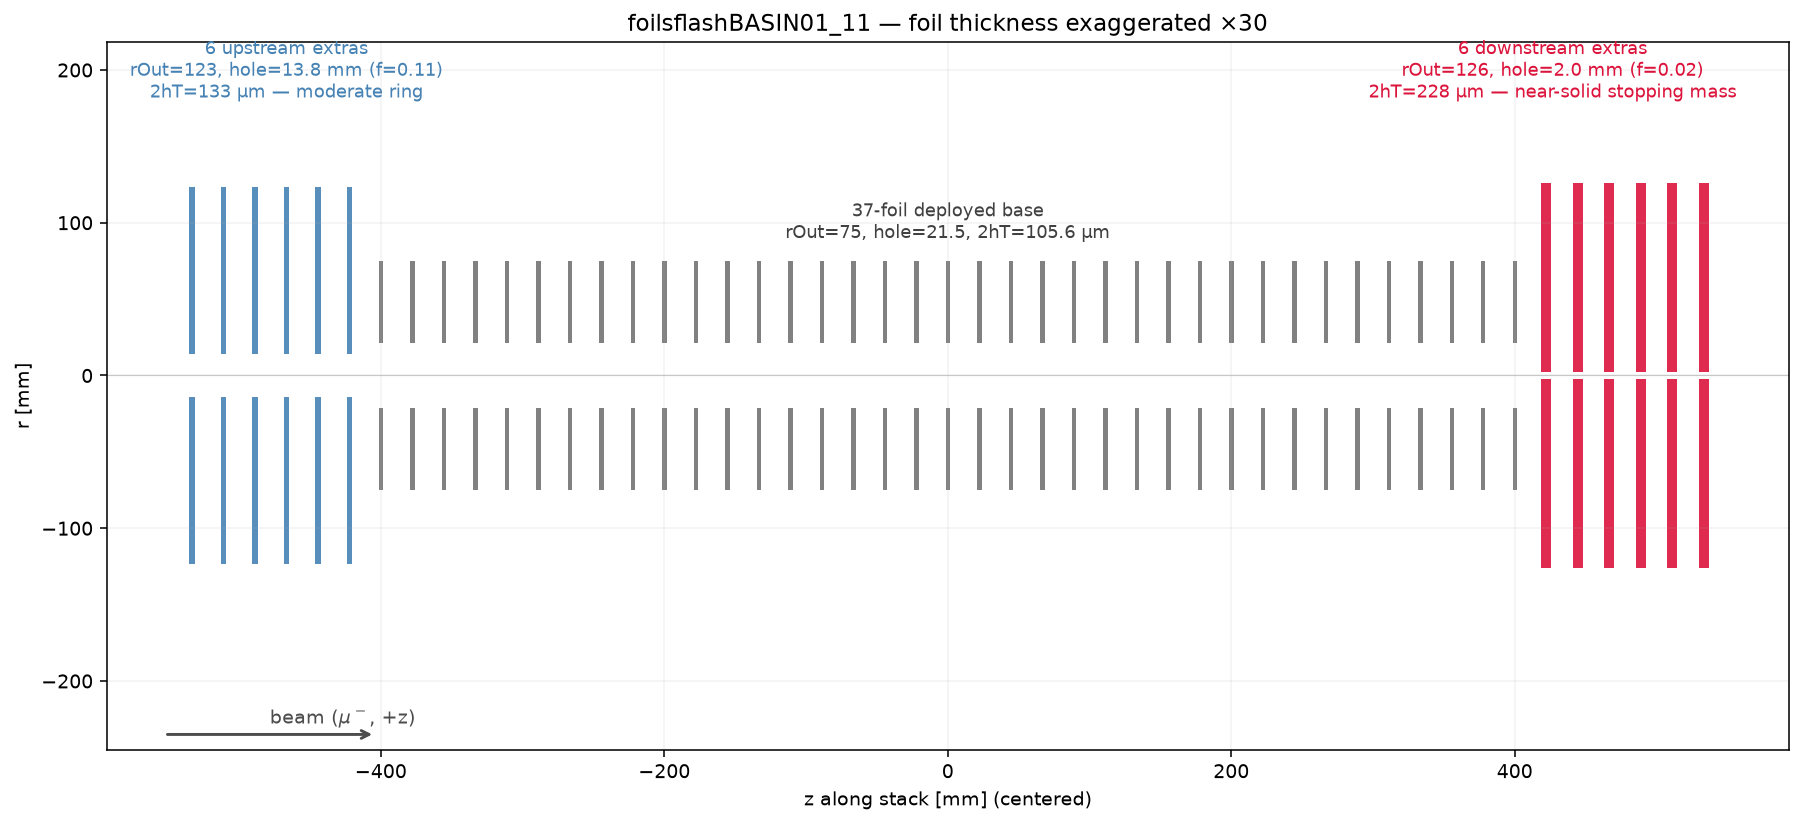
\includegraphics[width=0.92\textwidth]{foilsflash_bestsob_sketch.png}
\end{center}
\vspace{-0.2em}
\footnotesize
Two routes to high S/$\sqrt{B}$: a thin \textbf{off-beam ring}, or thin \textbf{in-beam}
material that degrades the beam to stop more muons. Here: 6 upstream extras (moderate ring)
$+$ 6 downstream (near-solid stopping mass) around the 37-foil deployed base.
\end{frame}

% --------------------------------------------------------------- milestones §4
\begin{frame}{Phase I milestones --- where Workflow (i) stands}
\small
9 months from \textbf{1 Aug 2026}; go/no-go at month 6 (Jan 2027). \textbf{We are in month 1.}
\vspace{0.6em}
\begin{center}
\scriptsize
\begin{tabular}{@{}llll@{}}
\hline
\textbf{window} & \textbf{dates} & \textbf{milestone (Workflow (i) parts)} & \textbf{status} \\
\hline
Months 1--2 & Aug--Sep 26 & Deploy interfaces: Simulation, Analysis, Documentation & \textcolor{red}{pending} \\
            &             & End-to-end agentic chain: sim $\rightarrow$ analysis $\rightarrow$ FoM & \textcolor{okgreen}{\textbf{done}} \\[0.3em]
Months 3--4 & Oct--Nov 26 & Exercise optimization on campaigns; collect metrics & \textcolor{okgreen}{\textbf{ahead}} \\[0.3em]
Months 5--6 & Dec--Jan 27 & Compile go/no-go results; \textbf{all traces logged} & \textcolor{red}{traces = gap} \\[0.3em]
Months 7--9 & Feb--Apr 27 & Harden interfaces; package artifacts for Genesis & --- \\
\hline
\end{tabular}
\end{center}
\vspace{0.6em}
\begin{itemize}\small
  \item One month in: the \textbf{science milestone of months 3--4 is already met}; interfaces are the open item
  \item Proposal \S4 anticipates this: \emph{``initial workflow prototyping can use simplified interfaces while production versions are improved''}
\end{itemize}
\end{frame}

% --------------------------------------------------------------- gate metrics
\begin{frame}{Decision gate metrics --- Workflow (i), proposal \S6}
\footnotesize
\scriptsize
\textbf{(a)} \emph{``Closed-loop sim--analysis--optimization (agent-orchestrated search with Bayesian
optimization for local sampling) demonstrated on $\ge$\,2 distinct external-constraint scenarios
(e.g.\ half beam intensity, 10\% reduced fields), each initiated by a natural-language prompt and
completed within one week (vs.\ months for the manual baseline), with full traces logged''}
\begin{itemize}\footnotesize
  \item[$\rightarrow$] \textbf{Started.} ``Optimize shape at the deployed foil pitch'' $\rightarrow$ new mode spec, validated geometry, 20 evaluations in \textbf{7.3 h} (2026-08-04 23:34 $\rightarrow$ 08-05 06:51)
  \item[$\rightarrow$] \textbf{20 evaluations suffice}: a cold-start line hit sob 4.09 by eval 16 --- matching a predecessor that took \textbf{414}. Saturation needs a second campaign ($+0.00$): a scenario answers \textbf{within a day} vs.\ a one-week bar
  \item[$\rightarrow$] Remaining: the two \textbf{external-constraint} scenarios --- reduced / absent DS field, half beam intensity --- and \textbf{formal trace logging}
\end{itemize}
\vspace{0.7em}

\textbf{(b)} \emph{``for a Run-1a scenario (no full cosmic ray veto coverage), starting from the
collaboration's existing manually-optimized baseline, agent-produced configuration achieves improved
$R_{\mu e}$ sensitivity, with improvements documented for collaboration review''}
\begin{itemize}\footnotesize
  \item[$\rightarrow$] \textcolor{okgreen}{\textbf{Demonstrated}}: champion beats the deployed target on \textbf{both} axes ($+6\%$ S/$\sqrt{B}$, $-3\%$ damage); $\mathbf{+25\%}$ S/$\sqrt{B}$ at the confirmed ceiling
  \item[$\rightarrow$] To finish: \textbf{prove it with full sims} (dig $\rightarrow$ mcs $\rightarrow$ nts) on the best configs
  \item[$\rightarrow$] Then: scope by background regime (part of the gain is Run-1a-specific); document for review
\end{itemize}
\end{frame}


% =========================================================== BACKUP
\begin{frame}[plain]
\vspace{2.5em}
\begin{center}
{\Large\bfseries\color{fnalblue} Backup}
\end{center}
\end{frame}

% ------------------------------------------------- what BO actually is
\begin{frame}{What ``GP surrogate $+$ multi-objective acquisition'' means}
\small
\textbf{GP surrogate --- the map.}
Each real evaluation costs $\sim$150 CPU-hours, so we cannot try many designs. The Gaussian
Process looks at every design tried so far and draws a map of the whole space: for a design we
have \emph{not} tried it predicts the answer \textbf{and how unsure it is}. Near measured points
the prediction is sharp; far away it is foggy. \emph{The fog is the useful part.}
\vspace{0.7em}

\textbf{Acquisition --- the rule for where to go next.}
Something has to choose which 10 designs to actually simulate next. The acquisition function
trades off \textbf{exploit} (go where the map predicts good results) against \textbf{explore}
(go where the fog is thick --- we might be missing something).
\vspace{0.7em}

\textbf{Multi-objective --- why there is no single ``best''.}
We want two things at once: more signal, less detector damage. They fight each other, so there
is no single winner --- there is a \textbf{set} of best compromises, the \textbf{Pareto front}
(the map on the status slide). Our acquisition function (\texttt{qNEHVI}) picks the designs
expected to push that frontier \emph{outward} the most, rather than chasing one number.
\end{frame}

\end{document}
